\section{Introduction: why the data source matters}
Volatility measures how strongly prices fluctuate. Researchers and investors often calculate a daily volatility estimate from prices observed during the trading day. That estimate can then enter a forecasting model or a rule for deciding how much to invest. It is therefore worth asking how the estimate depends on the data file used to construct it.

A trade file contains more than prices. It also records when trades occurred and attaches labels describing them. A program may keep some labels and reject others. If two sources store time or labels differently, applying the same filtering instruction can produce different retained observations. The resulting volatility estimates can differ even when the sources contain matching recorded prices, sizes and trading venues.

This paper asks: \emph{when the calculation rule stays fixed, how much does the representation of trade information change a volatility estimate and the investment amount calculated from it?} It also asks whether an upper limit on investment makes two different estimates appear to agree.

We use two historical trade-data representations available through Wharton Research Data Services (WRDS). One records time in seconds; the other records it in milliseconds. We compare the original representations and deliberately exchange their time and condition information. This helps locate which information matters within the chosen calculation. The exercise does not establish which source gives true volatility.

The connection to rough volatility concerns a separate distinction. Prices fluctuate, and the volatility of those fluctuations can itself change. Rough-volatility models describe particularly irregular changes in volatility over short time scales. Gatheral, Jaisson and Rosenbaum~\cite{gjr} provide influential evidence and modeling arguments for this idea. However, true volatility is hidden, so empirical work often studies estimates constructed from prices instead.

Cont and Das~\cite{contdas} show how an observed volatility estimate can look rough even when the underlying process is not rough. Fukasawa, Takabatake and Westphal~\cite{ftw} also study misleading effects of observation error, while developing a different estimation method whose empirical results still support rough volatility. The lesson is that measurement needs attention. These papers do not imply that every low roughness estimate must be an error.

Differences between historical trade databases are already known. Holden and Jacobsen~\cite{holden} document differences in liquidity measures across Monthly and Daily TAQ. VOLARE~\cite{volare} discusses source formats, trade timing and trade-size categories when constructing realized measures. This study does not claim to discover that data cleaning matters. It contributes a controlled historical example and follows the effect from the source fields through to a proposed investment.

The main findings are easy to state. Source information changes some daily measurements and the positions proposed from them. A common investment cap can hide much of the resulting difference. The size of the effect also depends on the fund: the relatively small five-minute position gaps for SPY do not carry over uniformly to QQQ. We report the complete fixed comparisons, including small effects and unavailable results.

\section{Data and comparison design}\label{sec:data}
\subsection{What is observed, and what is a fund-day?}
The funds in this study are exchange-traded funds (ETFs): funds whose shares can be traded on an exchange. SPY, QQQ, IWM, EFA and TLT are their trading symbols. Here they identify the assets whose records we compare; the study does not try to rank the funds as investments.

A \emph{fund-day} means one fund observed during one exchange session. A \emph{source-paired fund-day} means that its records are available in both representations and have passed the required correspondence checks. It is a unit of data coverage, not an independent experiment.

The original source study, labeled A10, covers \Fact{sessions} trading sessions for SPY from 2 January 2013 to 31 July 2014. It also includes QQQ, IWM, EFA and TLT for January 2014. That first export contains \Fact{symbolDays} fund-days and \Fact{records} matched ordered records before cleaning.

The word \emph{matched} needs care. We check whether the sources have corresponding recorded prices, sizes and venues in the required order. This is weaker than proving that every record represents a different economic trade. Repeated identical records can be difficult to distinguish. Matching also does not prove that either source records every trade perfectly.

A later fixed follow-up, A13, extends all four other funds to the same \BF{sessions}-session calendar. It adds \BF{newPairs} paired fund-days and reuses the \BF{reusePairs} January pairs already seen. The four-fund extension has \BF{pairs} pairs. Including SPY gives \BF{unionPairs} distinct fund-days, with reused observations counted once.

The historical window comes from the common period available in the mounted sources. Raw trade records are processed on WRDS rather than downloaded locally. Local files contain daily measures, checks and records of how the files were produced.

\subsection{Why some dates are excluded from some results}
The mechanism was first examined on two dates: 2 January 2014 and 3 July 2014. These are \emph{discovery dates}: observations that helped motivate the later comparison. Counting them as previously unseen evidence would overstate the strength of that comparison.

The main SPY count of affected dates therefore excludes these two dates, leaving \Fact{den60} eligible source pairs at one minute. The four-fund follow-up also excludes the January 2014 month, because that panel had already been examined. Its main calendar has \BF{eligible} eligible dates per fund before any missing measurements. Consequently, the main SPY and follow-up counts have different denominators.

Other calculations ask about a complete history rather than the count on new eligible dates. The descriptive roughness summaries and the smoothed risk rule retain the full calendar, including discovery dates. Removing dates would change the time gaps and the memory of the rule. Each table states which sample it uses.

The design was recorded before each expanded run, but earlier results had already influenced the research question. The follow-up is therefore exploratory historical evidence. It is not untouched chronological validation. Validation observations from 2017--2019 and final observations from 2020 onward remain closed.

\subsection{Changing time and trade labels separately}
The reference, written $M$, uses modern time and modern trade-condition labels. The legacy comparison, $L$, uses legacy time and legacy labels. We also run three mixed constructions. One combines modern time with legacy labels. Another combines legacy time with modern labels. The third keeps legacy time and labels but restores modern category-B information.
The rest of the calculation stays fixed. This is a controlled change in the information supplied to the program, rather than a claim about economic causality.

Category B is one of the trade-condition categories. Its documented meaning differs by reporting tape: it denotes average-price trades for CTA issues and bunched trades for UTP issues~\cite{nyse}. A reporting tape is a system for consolidating trade reports. We should therefore not attach one economic meaning to B across all funds.

Restoring B information asks whether that missing information explains a discrepancy in this particular calculation. It does not recommend removing every B-coded trade or adopting the restoration as a general cleaning rule. Direct checks of time rounding and correction fields were also made on the two discovery dates; we do not claim that this stronger field-level check was repeated on every date.

\begin{figure}[H]
\centering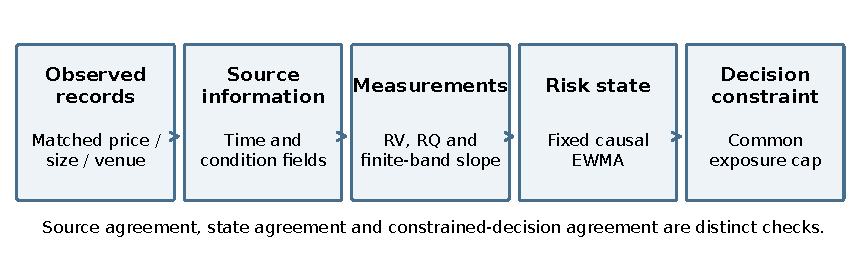
\includegraphics[width=\linewidth]{figures/workflow.pdf}
\caption{The steps being checked. Recorded trades supply time and condition information. That information enters daily measurements, which enter a smoothed risk estimate and a proposed investment subject to a cap. Matching a later step does not prove that the earlier steps match. This is a calculation chain, not a model of economic cause and effect.}\label{fig:workflow}
\end{figure}

\section{How the measurements and investment rule work}\label{sec:methods}
\subsection{Selecting prices during a session}
A trading session is the exchange's open-to-close period. The pipeline first keeps observations with positive finite prices and sizes during that session, applies its rule for uncorrected trades, and retains only condition strings that are blank or contain the regular-trade symbol @ after whitespace normalization.

It then chooses the venue with the largest retained trade count. A venue is an exchange or other trading location. Ties are broken by venue identifier. If several retained prices have the same timestamp, the median price is used. These choices are held fixed across the source constructions.

Next, the program selects prices on six schedules: every 15 seconds, 30 seconds, one minute, five minutes, 15 minutes and 30 minutes. At each scheduled point, it uses the most recent eligible recorded price. This is called \emph{previous-tick sampling}; a tick here is a recorded trade observation.

There is a special rule at the opening point. If no retained trade occurs exactly at the open, the first eligible trade supplies an approximate opening anchor, and the approximation is flagged. Later empty grid points are not filled backwards from a future observation. If a required grid is incomplete, its measurements remain missing. A missing part of the day is not treated as a complete shorter day.

The strict blank-or-@ filter is intentional: it tests what happens when the same literal instruction meets different source information. It retains fewer condition types than the inspected \texttt{highfrequency} cleaner and also differs in the order of venue selection~\cite{highfrequency}. This is not a full comparison of cleaning packages, nor a full replication of a general BNHLS cleaning procedure.

\subsection{Returns, realized variance and quarticity}
For prices $P_{\rm old}$ and $P_{\rm new}$, the log return is
\[
 r=\log(P_{\rm new}/P_{\rm old}).
\]
Here $\log$ is the natural logarithm. For small price changes, the log return is close to the ordinary percentage change written as a decimal, but they are not exactly equal.

Let $t$ label the session and $i$ label an interval within it. Let $M_t$ be the actual number of sampled return intervals in that complete session. Realized variance (RV) adds squared log returns:
\begin{equation}
 \RV_t=\sum_{i=1}^{M_t}r_{t,i}^2,\qquad
 \RQ_t=\frac{M_t}{3}\sum_{i=1}^{M_t}r_{t,i}^4.\label{eq:moments}
\end{equation}
The symbol $\sum$ means to add the contribution from each interval. Squaring makes both positive and negative returns contribute positively. Realized quarticity (RQ), the second expression, uses fourth powers and therefore gives relatively more weight to large movements.

\textbf{Worked example, using invented log returns.} Suppose a simplified session has three returns: $0.01$, $-0.01$ and $0.02$. Then
\[
 \RV=0.01^2+(-0.01)^2+0.02^2=0.0006,
 \qquad \sqrt{\RV}\simeq 0.0245=2.45\%.
\]
The square root gives a volatility-scale measure of the movements during this invented session. It is not the session's return. Its quarticity is
\[
 \RQ=\frac{3}{3}\left(0.01^4+(-0.01)^4+0.02^4\right)
     =0.00000018.
\]
Doubling one return multiplies its squared contribution by four and its fourth-power contribution by sixteen. That explains why RQ can respond strongly to isolated large increments. It does not guarantee that the source difference in RQ is always larger than the source difference in RV.

The factor $M_t/3$ has a mathematical basis. Under an ideal model with independent normal price increments and stated assumptions about the variance path, the fourth moment of a standard normal variable is three. Appendix~\ref{app:moments} derives the normalization carefully. Those assumptions are an explanation of the formula, not a claim that the historical trade data exactly satisfy that model.

The exchange calendar supplies the session length, including early closes, so $M_t$ follows the actual session. Returns are in decimal units and are not annualized at this stage. The measure covers the session and excludes a separately constructed overnight return. Changing decimal returns to percent returns multiplies RV by $100^2$ and RQ by $100^4$. Units and time coverage must agree before two estimates can be compared.

\subsection{When does a source difference count as material?}
For a positive valid pair, divide the candidate measurement by the modern reference. A ratio of one means agreement. RV is called \emph{materially different} when the ratio is greater than 1.1 or smaller than $1/1.1$. RQ uses the wider limits 2 and $1/2$.

For example, invented RV values of 100 and 105 do not pass the RV threshold. Values of 100 and 111 do. A ratio of exactly 1.1 is on the boundary and does not pass the strict threshold. The reciprocal lower limit keeps the decision the same if the two sources exchange places.

For computation, we write the same rule with a log ratio:
\[
 d_{t,Q}=\log(Q_t^{\rm candidate}/Q_t^M),
 \quad |d_{t,\RV}|>\log(1.1),\quad |d_{t,\RQ}|>\log 2.
\]
Here $Q$ means either RV or RQ, and vertical bars mean absolute value. These are predefined practical thresholds. Passing one is not the same as statistical significance, and failing one does not establish that two sources are equivalent.

An entry such as $41/396$ means 41 material dates out of 396 valid eligible source pairs. The term \emph{incidence} in a table means this fraction of affected dates. A missing pair is excluded from the valid denominator and never counted as agreement.

\subsection{A descriptive summary of changes across days}
We also ask how daily RV changes over different time gaps. Write $x_t=\log\RV_t$. A lag of one means comparing neighboring trading sessions; a lag of five means comparing sessions five trading days apart.

For each lag $k$, calculate the average squared change:
\begin{equation}
 \widehat V(k)=\frac{1}{|\mathcal I_k|}
       \sum_{t\in\mathcal I_k}(x_t-x_{t-k})^2,\qquad
 \widetilde H_K=\frac12\operatorname{slope}_{k=1,\ldots,K}
       \{\log k,\log\widehat V(k)\}.\label{eq:H}
\end{equation}
The set $\mathcal I_k$ contains dates whose two required RV values are valid; $|\mathcal I_k|$ is their count. Thus the first formula says: take the squared change for every valid pair at that lag and average those changes.

The second formula fits a straight line to log average squared change against log lag and takes half its slope. We call the result H-tilde, $\widetilde H$. The main calculation uses lags 1--10; fixed alternatives use 1--5 and 1--22. This limited range is what \emph{finite band} means.

\textbf{A two-lag illustration.} If the average squared change doubles when the lag doubles, the log-log slope is one, so H-tilde is one half. If the averages barely increase, the slope is much smaller. This illustration explains the calculation; the reported study uses the stated full lag ranges.

A smaller slope can have several explanations. One is how the underlying volatility changes. Another is measurement error in daily RV. For example, error at both endpoints can add a roughly constant amount to squared changes, making short-lag changes large relative to longer-lag changes. Appendix~\ref{app:noise} derives this under explicit assumptions.

The reported slopes do not identify latent market roughness. Here \emph{latent} means hidden: the true volatility process is not observed. Our statistic summarizes a finite set of daily RV changes. It is not Cont and Das's normalized variation estimator or Fukasawa et al.'s quasi-likelihood estimator, so theorems about those estimators are not transferred to it.

Missing dates retain their place on the calendar. Dropping one and treating its neighbors as consecutive would change the meaning of the lag. When comparing slopes across sources, the paired contrasts also use common valid endpoints so that support differences are visible.

\subsection{A risk estimate that remembers previous days}
To see whether daily source differences matter later, we use one fixed investment rule. It starts with a smoothed daily variance estimate, $s_t$. The update is an exponentially weighted moving average (EWMA):
\[
 s_0=\RV_0,\qquad s_t=\lambda s_{t-1}+(1-\lambda)\RV_t.
\]
With the original choice $\lambda=0.94$, the rule combines 94\% of the previous estimate with 6\% of today's RV. Repeated updating gradually reduces the influence of older observations.

\textbf{Worked example, using invented variance values.} If the previous estimate is $0.0001$ and today's RV is $0.0004$, then
\[
 s_t=0.94(0.0001)+0.06(0.0004)
     =0.000094+0.000024=0.000118.
\]
A single large source discrepancy can therefore affect many later estimates, even after that day's direct observation has passed. It is important to distinguish one persistent episode from many independent new shocks.

The estimate is initialized at the first day's RV. The first 126 observations are used as a warmup and excluded from the reported evaluation count. This leaves $\Fact{sessions}-126=\Fact{origins}$ evaluation dates. Complete positive history is required. Missing days are not filled or removed merely to make the update run.

\subsection{From estimated variance to a proposed investment}
The investment rule aims at a specified volatility target. Let $v_*$ denote that target, and let $c$ denote the position cap. It calculates an uncapped amount $u_t$ and then applies the cap:
\begin{equation}
 s_0=\RV_0,\quad s_t=\lambda s_{t-1}+(1-\lambda)\RV_t,\qquad
 u_t=\frac{v_*}{\sqrt{252s_t}},\qquad
 w_{t+1|t}=\min(c,u_t).\label{eq:weight}
\end{equation}
The first part repeats the estimate update so that the full rule is shown together. The factor 252 is the fixed annualization convention: daily variance is multiplied by it, then square-rooted to obtain an annual volatility estimate. The target divided by that estimate gives the proposed share of capital. If estimated volatility rises, the proposed position falls.

The function $\min(c,u_t)$ takes the smaller of the cap and the uncapped proposal. Original settings are $\lambda=0.94$, target $v_*=0.10$ and cap $c=1$. The target therefore means 10\% annual volatility under this convention, and the cap means at most 100\% of capital in the fund.

Continuing the invented variance example gives
\[
 \sqrt{252(0.000118)}\simeq0.1724=17.24\%,\qquad
 u_t=\frac{0.10}{0.1724}\simeq0.580.
\]
The rule proposes approximately 58.0\% of capital. A 100\% cap leaves that proposal unchanged. If two source estimates instead both produced proposals above 100\%, the cap would make both final positions equal 100\%.

The notation $w_{t+1|t}$ means the proposal for the next session based on information available by the end of session $t$. An \emph{origin} is that information date, not an independent event. The same session's full RV is never used before the session finishes.

The analysis does not evaluate returns, transaction costs or profit. It compares proposed inputs to a rule. The annualization convention also does not turn open-to-close RV into a complete measure of actual overnight-inclusive portfolio risk. Appendices~\ref{app:state}--\ref{app:weights} give the exact memory and cap calculations.

A predefined warning criterion is met if at least 2\% of valid non-discovery dates are material at a grid, or at least ten evaluated origins have a position difference of at least 5pp. This flags practical sensitivity in the pipeline. It is not a test of originality or proof that one source is more accurate.

\subsection{Uncertainty and checks of alternative settings}
Neighboring dates may share market conditions or the same persistent source effect. Treating every date as independent would misrepresent how much separate evidence the sample contains. The uncertainty calculation therefore resamples blocks of dates while keeping the source pair together~\cite{politis}.

The stationary bootstrap used here starts at random dates and forms stretches of neighboring dates with random lengths. It repeats the sample construction 3,999 times and recalculates the fraction of material dates each time. Mean block length 22 is the main choice; 11 and 44 are fixed alternatives. All funds use the same resampled date indices, preserving their common calendar dependence.

The displayed intervals summarize variation across these resamples. They rely on the historical window being sufficiently representative and its dependence being compatible with the resampling method. They do not create new market episodes, prove source equivalence or guarantee accuracy after a change in the data-generating regime.

After seeing the original SPY results, the A11 exercise fixes 27 combinations of memory, target and cap:
\[
 \lambda\in\{.90,.94,.97\},\qquad
 v_*\in\{.05,.10,.15\},\qquad c\in\{.5,1,2\}.
\]
There are $3\times3\times3=27$ combinations. They are all reported. The exercise is \emph{post-result}: its question was chosen after the original results. It is a sensitivity check and not a new confirmatory sample.

Two useful identities are
\begin{equation}
 \frac{u_t^L}{u_t^M}=\sqrt{\frac{s_t^M}{s_t^L}},
 \qquad |\min(c,a)-\min(c,b)|\leq |a-b|.\label{eq:cap}
\end{equation}
The first says that the ratio between uncapped proposals depends only on the ratio between their variance estimates: the common target and annualization factor cancel. The second says that applying the same upper cap cannot enlarge a difference. It can shrink that difference, sometimes all the way to zero. Section~\ref{sec:cap} uses these facts to interpret the findings.

\section{Simulation: a setting where true volatility is known}\label{sec:simulation}
In real trade data we cannot observe the true volatility path directly. A simulation gives a different kind of evidence: we choose a mathematical process, generate artificial observations from it, and know which process produced them. We can then examine what the measurement procedure reports.

The simulation separates three objects. A spot sample is the model's variance at a point in time. Integrated variance adds up variance during a session; its grid approximation uses the average of fine-step variance values on a session clock of length one. RV is then calculated from the artificial price returns. These objects are related, but they are not interchangeable observations.

One model is Ornstein--Uhlenbeck (OU), which fluctuates around a long-run level and has exponentially declining dependence across time. Two further Gaussian models use a generalized Cauchy covariance with local roughness parameters $H=.1$ and $.3$, following the covariance family discussed by Bennedsen, Lunde and Pakkanen~\cite{blp}. They are not claimed to be fractional OU processes. The OU model's local roughness exponent is $.5$; this describes its behavior at sufficiently small time scales, not every finite-lag statistic.

For reproducibility, log variance $X$ is converted to positive variance by $v_t=10^{-4}\exp(X_t-0.25/2)$. The OU covariance is $0.25\exp(-\kappa|h|)$, where $h$ is a time gap and $\kappa=\log(2)/22$. All settings share the stated 22-day half-correlation scale. This fixes how quickly model dependence declines.

For each model, 128 independent artificial histories contain 504 sessions with 780 fine steps per session. Model variance generates normally distributed price increments conditional on that variance path. Independent log-price noise of 0, 1 or 3 basis points is added at fine-grid price endpoints. A basis point is one hundredth of a percentage point. Coarser returns come from the same underlying fine path, using intervals of 1, 5, 15 and 30 minutes.

The important result is that the same generating process gives different descriptive slopes at different observation stages. Without added price noise, the OU case has mean H-tilde \Fact{ouSpot} for spot samples, \Fact{ouIV} for grid-integrated variance and \Fact{ouRV} for five-minute RV. The Monte Carlo standard error of the last mean is \Fact{ouSE}; it measures simulation sampling uncertainty across the independent artificial histories.

\begin{figure}[H]
\centering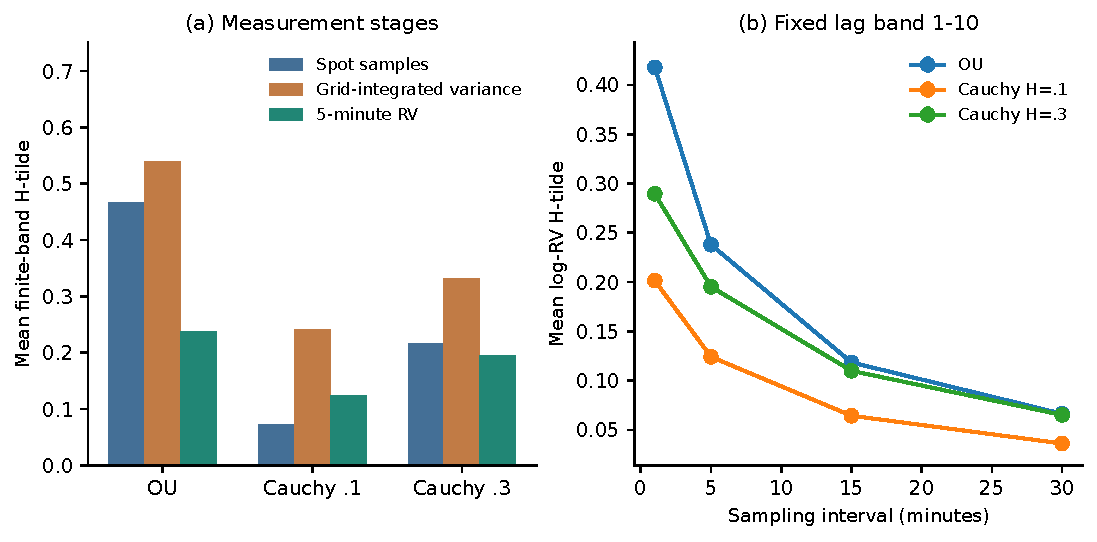
\includegraphics[width=\linewidth]{figures/synthetic.pdf}
\caption{The simulation illustrates the effect of measurement. Panel (a) starts with the same model but compares spot samples, grid-integrated variance and five-minute RV. Panel (b) changes the price-sampling interval. All slopes use daily lags 1--10. Error bars show simulation uncertainty across independent paths, not confidence intervals for real market roughness. No log-price noise is added in this displayed comparison; other fixed settings remain in the supporting tables. Source: A08.}\label{fig:synthetic}
\end{figure}

Thus a low slope from observed RV does not by itself reveal the model's local roughness parameter. This is consistent with the measurement concerns in the literature~\cite{contdas,ftw}. The simulation is a controlled illustration, not an estimate of the hidden process behind SPY and not a refutation of rough-volatility models.

\section{Results for SPY}\label{sec:results}
\subsection{Daily measurement differences}
At one minute, legacy RV differs materially from modern RV on \Fact{rvN60} of \Fact{den60} valid non-discovery dates. RQ differs materially on \Fact{rqN60} of \Fact{den60}. The main block-resampling intervals for the affected fractions are \Fact{RVlower}--\Fact{RVupper}\% for RV and \Fact{RQlower}--\Fact{RQupper}\% for RQ.

\begin{table}[H]
\centering\small\setlength{\tabcolsep}{4pt}
\caption{SPY at every fixed sampling interval. RV and RQ entries give affected dates / valid dates, excluding the two discovery dates. H-tilde summarizes the full calendar using lags 1--10. Mean position gaps and counts of origins with a gap of at least 5pp use the original investment rule and \Fact{origins} evaluation dates.}\label{tab:grid}
\begin{tabular}{lrrrrrr}
\toprule
Grid & RV material & RQ material & $\widetilde H_M$ & $\widetilde H_L$ & Mean gap (pp) & $\geq5$pp origins \\
\midrule
15s & \Fact{rvN15}/\Fact{den15} & \Fact{rqN15}/\Fact{den15} & \Fact{hM15} & \Fact{hL15} & \Fact{gap15} & \Fact{large15} \\
30s & \Fact{rvN30}/\Fact{den30} & \Fact{rqN30}/\Fact{den30} & \Fact{hM30} & \Fact{hL30} & \Fact{gap30} & \Fact{large30} \\
1m & \Fact{rvN60}/\Fact{den60} & \Fact{rqN60}/\Fact{den60} & \Fact{hM60} & \Fact{hL60} & \Fact{gap60} & \Fact{large60} \\
5m & \Fact{rvN300}/\Fact{den300} & \Fact{rqN300}/\Fact{den300} & \Fact{hM300} & \Fact{hL300} & \Fact{gap300} & \Fact{large300} \\
15m & \Fact{rvN900}/\Fact{den900} & \Fact{rqN900}/\Fact{den900} & \Fact{hM900} & \Fact{hL900} & \Fact{gap900} & \Fact{large900} \\
30m & \Fact{rvN1800}/\Fact{den1800} & \Fact{rqN1800}/\Fact{den1800} & \Fact{hM1800} & \Fact{hL1800} & \Fact{gap1800} & \Fact{large1800} \\
\bottomrule
\end{tabular}

\end{table}

At five minutes, RV still differs materially on \Fact{rvN300} dates, while RQ differs on fewer dates. Coarser sampling therefore does not remove every daily discrepancy. The table also shows why one should report every chosen interval: the count does not simply fall as the interval becomes wider.

The one-minute H-tilde values are \Fact{hM60} with modern information and \Fact{hL60} with legacy information. Restoring B information gives \Fact{hB60}. These are descriptions of the constructed RV series. They are not estimates that identify the hidden market process. Appendix~\ref{app:bands} includes the other fixed lag ranges so that the interpretation does not depend on one selected band.

\begin{figure}[H]
\centering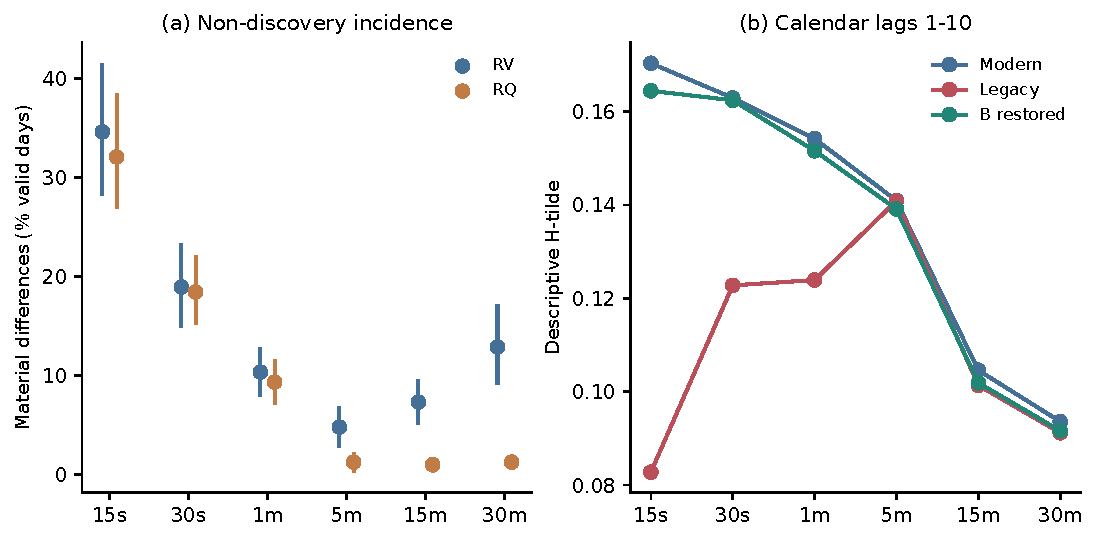
\includegraphics[width=\linewidth]{figures/measurement.pdf}
\caption{Two different summaries of the SPY comparison. Panel (a) gives the percentage of valid non-discovery dates with material RV or RQ differences and the main block-resampling intervals. Panel (b) gives full-calendar H-tilde, including discovery dates. The panels use different sample rules because they answer different questions. The slopes describe estimated RV rather than true market roughness. Source: A10.}\label{fig:measurement}
\end{figure}

\subsection{What changes when time and labels are exchanged?}
The crossed constructions help locate the discrepancy. Keeping legacy labels while restoring precise time still leaves \Fact{crossRV1} material one-minute RV dates. Keeping legacy time but using modern labels reduces that count to \Fact{crossRV2}. Restoring B information under legacy time and the other legacy labels leaves \Fact{crossRV3}.

\begin{table}[H]
\centering\small\setlength{\tabcolsep}{5pt}
\caption{Changing time and condition information separately for SPY at one minute. Every comparison uses the modern reference and \Fact{den60} valid non-discovery dates. The modern reference compared with itself has zero differences by construction.}\label{tab:cross}
\begin{tabular}{lrrr}
\toprule
Construction & RV material & RQ material & Mean abs. log RV ratio \\
\midrule
Legacy time / legacy flags & \Fact{crossRV0} & \Fact{crossRQ0} & \Fact{crossLog0} \\
Modern time / legacy flags & \Fact{crossRV1} & \Fact{crossRQ1} & \Fact{crossLog1} \\
Legacy time / modern flags & \Fact{crossRV2} & \Fact{crossRQ2} & \Fact{crossLog2} \\
Legacy + B information & \Fact{crossRV3} & \Fact{crossRQ3} & \Fact{crossLog3} \\
\bottomrule
\end{tabular}

\end{table}

Within this pipeline, time precision alone therefore explains much less than the available condition information. This is a limited conclusion about the program and source fields. Changing which trades pass a filter can also change the chosen venue and the median price at a timestamp. The effects need not add up as separate economic causes.

The first one-month panel was a small check beyond SPY. After excluding its January discovery date, one-minute RV counts are \Fact{panelEFArv}/\Fact{panelEFArvden} for EFA, \Fact{panelIWMrv}/\Fact{panelIWMrvden} for IWM, \Fact{panelQQQrv}/\Fact{panelQQQrvden} for QQQ and \Fact{panelTLTrv}/\Fact{panelTLTrvden} for TLT. Corresponding RQ counts are \Fact{panelEFArq}/\Fact{panelEFArqden}, \Fact{panelIWMrq}/\Fact{panelIWMrqden}, \Fact{panelQQQrq}/\Fact{panelQQQrqden} and \Fact{panelTLTrq}/\Fact{panelTLTrqden}. These funds share dates, so their observations are not pooled as independent experiments. Section~\ref{sec:breadth} reports the much longer fixed follow-up.

\subsection{How daily differences affect later proposed positions}
Under the original rule, the mean absolute one-minute position gap is \Fact{gap60}pp and the maximum is \Fact{maxGap}pp. Absolute means that we measure the size of a gap regardless of which source proposes the larger amount, then average those sizes.

A gap of at least 5pp occurs on \Fact{large60} of \Fact{origins} evaluation dates. Those dates form one consecutive episode, from 23 January to 31 March 2014. They are not \Fact{large60} independent new shocks. The EWMA remembers previous differences, so one period of source disagreement can affect many successive proposals. Restoring B information reduces the mean one-minute gap to \Fact{restoreGap}pp under this particular rule.

\begin{figure}[H]
\centering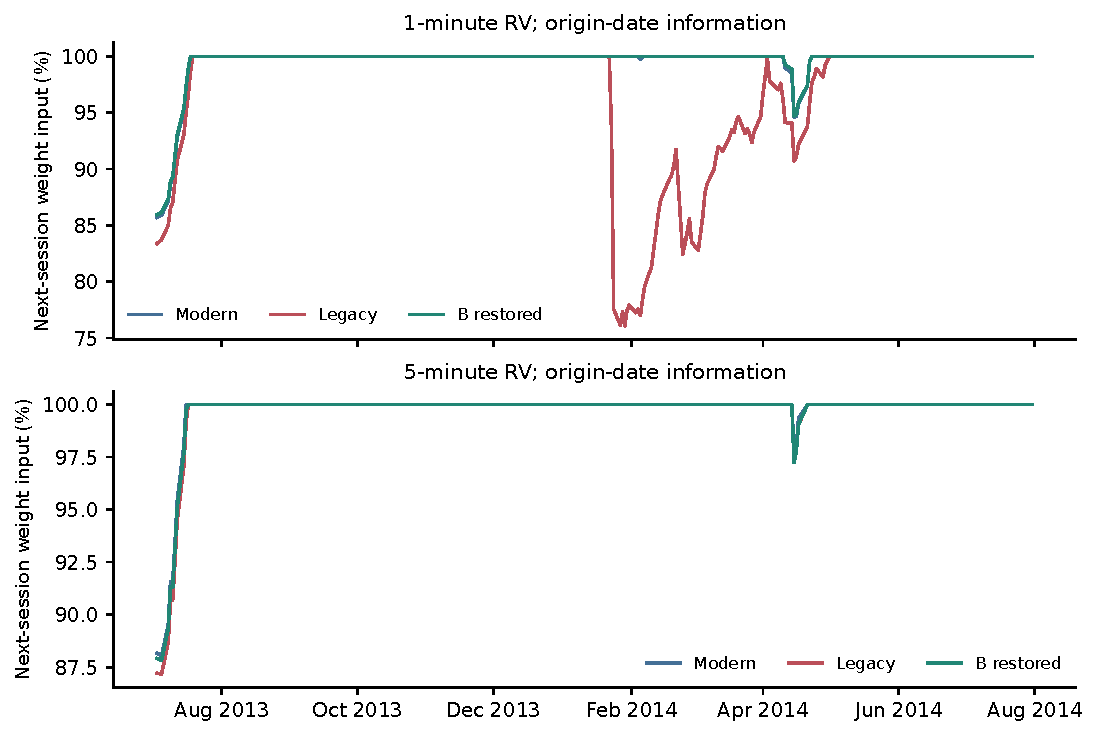
\includegraphics[width=.96\linewidth]{figures/weight_paths.pdf}
\caption{Proposed positions from the original rule: memory $\lambda=.94$, target 10\%, cap 100\% and a 126-observation warmup. Dates on the horizontal axis identify the completed session supplying information for the next proposal. The one-minute legacy series differs over one persistent episode. The five-minute capped positions look closer, but Section~\ref{sec:cap} checks whether the cap hides disagreement. These are proposed weights, not realized investment returns. Source: A10.}\label{fig:paths}
\end{figure}

A further post-result check replaces the legacy RV effect on the two discovery dates with the corresponding modern values. It keeps the dates in place. There are still \Fact{discoveryStandardized} origins with a gap of at least 5pp. Separately omitting those dates' increment endpoints gives approximate one-minute slopes of \Fact{discoveryHmodern} modern and \Fact{discoveryHlegacy} legacy. The full result is therefore not entirely due to those two observations. Because the check followed the result, it is a sensitivity exercise rather than independent confirmation or a proposed outlier-cleaning rule.

\section{Why a cap can hide disagreement}\label{sec:cap}
\subsection{A small final gap can come from the common limit}
For SPY at five minutes, the mean capped position gap is \Fact{gap300}pp. Before the cap, it is \Fact{uncapped300}pp. Both source proposals hit the cap on \Fact{bothCap300}\% of evaluated dates. The cap removes \Fact{attenuation300}\% of the uncapped mean gap. At one minute it removes \Fact{attenuation60}\%.

The calculation is
\[
 \text{fraction of mean gap removed}
 =1-\frac{\text{mean capped absolute gap}}
          {\text{mean uncapped absolute gap}},
\]
when the denominator is positive. It compares mean gap sizes before and after the cap. A large percentage should be read alongside the size of the uncapped gap; it does not measure an investment loss.

\begin{figure}[H]
\centering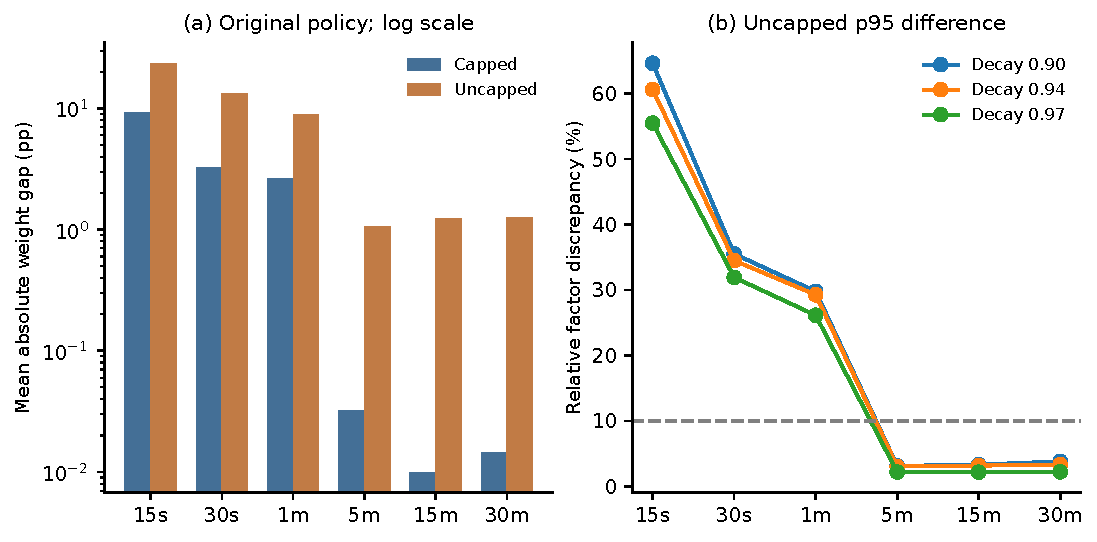
\includegraphics[width=\linewidth]{figures/cap_masking.pdf}
\caption{How the cap changes the SPY comparison. Panel (a) shows mean absolute position gaps before and after the cap; its vertical axis is logarithmic, so equal vertical distances mean equal multiplicative changes. Panel (b) summarizes relative uncapped proposal differences at three memory settings. Its p95 is the sample 95th percentile, a description of the observed values rather than an uncertainty interval. Source: A11, chosen after the original result.}\label{fig:cap}
\end{figure}

This does not mean that the observed difference between one- and five-minute sampling disappears when the cap is removed. At one minute, uncapped proposals differ by a factor above 1.1 on \Fact{relativemin60}--\Fact{relativemax60} of \Fact{origins} dates across the three memory settings. At five minutes those counts are zero for SPY. The uncapped ratio removes the common target and annualization factor, so it adds useful information about the relative variance estimates. It still does not tell us which estimate is true or what will happen in a future period.

\subsection{All fixed rule settings are retained}
A policy in this exercise means a specified memory, target and cap. Across all 27 fixed combinations, at least ten origins have a gap of 5pp or more in \Fact{policyLarge60} one-minute policies and \Fact{policyLarge300} five-minute policies. Some policies have zero capped gaps because both proposals reach the same cap.

\begin{figure}[H]
\centering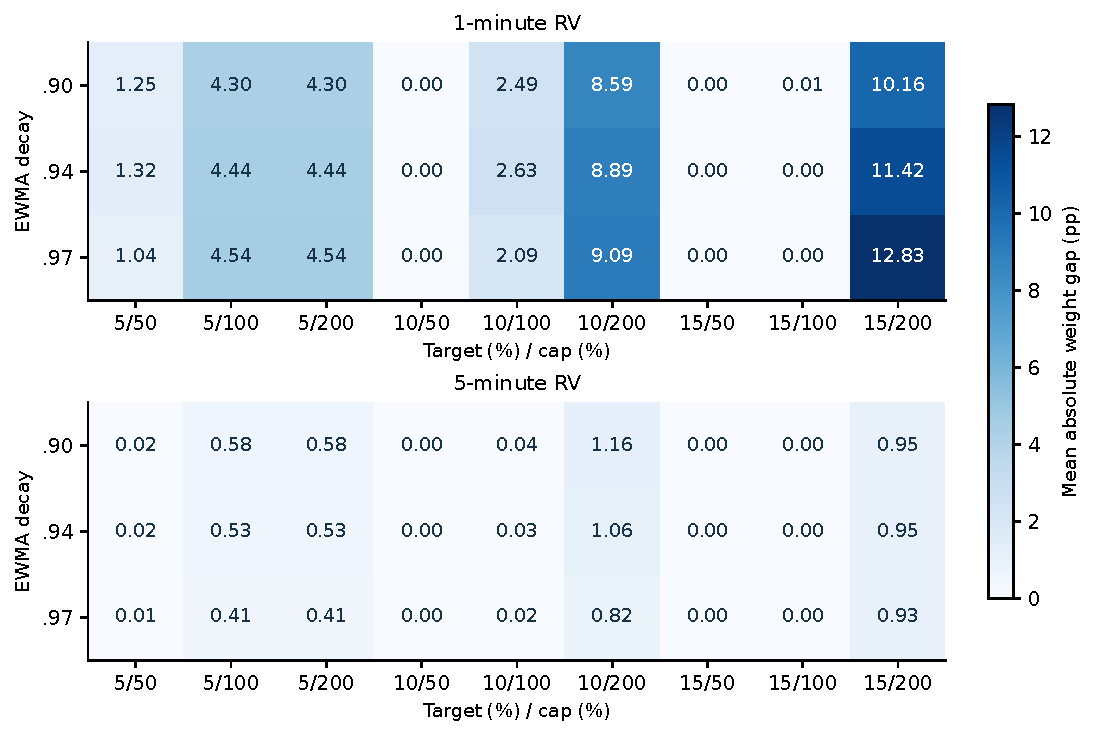
\includegraphics[width=\linewidth]{figures/policies.pdf}
\caption{Every fixed combination of memory, target and cap at one and five minutes. Each cell gives the mean absolute position gap in percentage points. Both panels use the same color scale. A colored cell describes one specified scenario; it does not identify a selected or optimal investment strategy. Source: A11.}\label{fig:policies}
\end{figure}

Appendix~\ref{app:policies} gives the complete table. These policies share data and formulas. They provide sensitivity information, not 27 independent confirmations, and none is selected as best.

An additional calculation asks how concentrated the possible persistence of daily differences is. At memory .94, the largest date accounts for \Fact{top_one_potential_share}\% of the absolute propagation-potential total, and the five largest account for \Fact{top_five_potential_share}\%. This calculation adds magnitudes to form an upper-bound measure; signed effects can partly cancel in the actual estimated state. The percentages therefore do not allocate actual investment losses or count independent economic shocks. Appendix~\ref{app:state} gives the mathematical definition.

\subsection{What changes when four more funds are examined?}\label{sec:breadth}
The follow-up extends QQQ, IWM, EFA and TLT to the same \BF{sessions}-session calendar as SPY. It adds \BF{newPairs} paired fund-days and reuses the \BF{reusePairs} January observations already examined. That gives \BF{pairs} pairs for the four funds and \BF{unionPairs} distinct fund-days including SPY.

The follow-up plan was fixed before downloading the additional observations, but after the SPY result was known. This is an exploratory follow-up, not untouched chronological validation. It expands the set of funds within one historical period.

The main count of affected dates excludes the previously seen January 2014 panel and the two discovery dates. That leaves \BF{eligible} eligible sessions per fund before missing measurements. The full-calendar slopes and smoothed risk calculations retain those dates to preserve time spacing and memory. The same date indices are used when resampling all funds. Shared dates are not treated as independent evidence merely because several funds are observed.

\begin{figure}[H]
\centering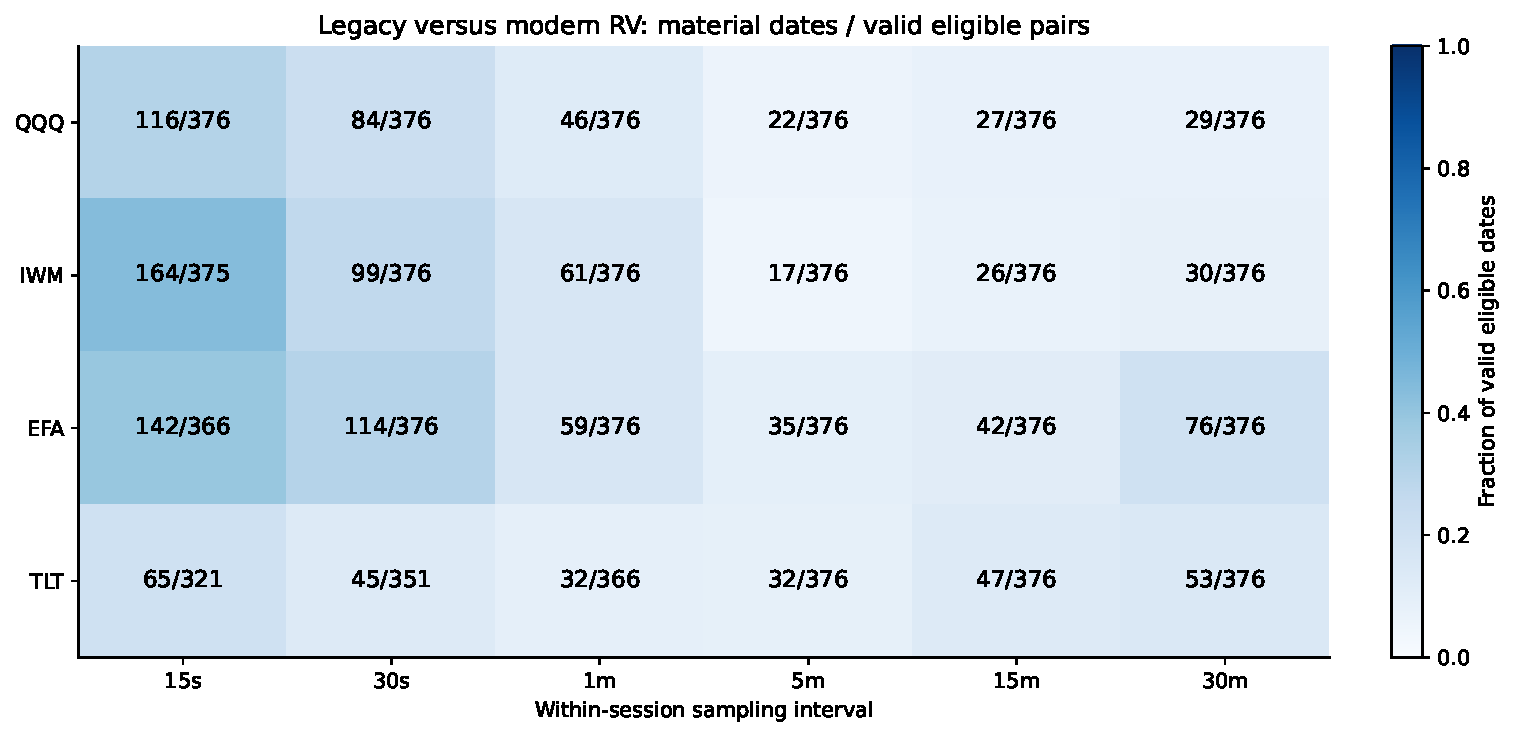
\includegraphics[width=\linewidth]{figures/breadth_incidence_rv.pdf}
\caption{Affected RV dates for every fund and sampling interval in the follow-up. Each cell gives affected dates / valid eligible pairs. Darker cells mean a larger affected fraction; the shared color scale runs from zero to one. The RV ratio must lie outside $[1/1.1,1.1]$ to count as material. Previously seen January dates and discovery dates are excluded. A missing pair does not count as agreement.}\label{fig:breadth-incidence}
\end{figure}

\textbf{How to read the complete comparison.} Table~\ref{tab:breadth-risk} places the daily measurement counts next to the later position differences. These answer different questions. RV/RQ counts concern individual eligible dates. Position gaps use the full chronological history and are evaluated after the warmup. A daily measurement difference can affect later proposals because the rule remembers past RV.

\begin{table}[H]\centering\small
\caption{All four follow-up funds at one and five minutes under the original rule. RV/RQ entries are affected dates / valid eligible dates. Capped and uncapped columns give mean absolute position gaps in percentage points. The final column counts evaluation dates with a capped gap of at least 5pp. Complete histories have \Fact{origins} evaluation dates. \emph{Withheld} means that the required TLT history is incomplete; it does not mean a zero effect.}\label{tab:breadth-risk}
\begin{tabular}{llrrrrr}\toprule
Fund & Grid & RV hits/valid & RQ hits/valid & Capped pp & Uncapped pp & Large origins \\ \midrule
QQQ & 1m & \BF{QQQ60LRVN}/\BF{QQQ60LRVD} & \BF{QQQ60LRQN}/\BF{QQQ60LRQD} & \BF{QQQ60capped} & \BF{QQQ60uncapped} & \BF{QQQ60large} \\
QQQ & 5m & \BF{QQQ300LRVN}/\BF{QQQ300LRVD} & \BF{QQQ300LRQN}/\BF{QQQ300LRQD} & \BF{QQQ300capped} & \BF{QQQ300uncapped} & \BF{QQQ300large} \\
IWM & 1m & \BF{IWM60LRVN}/\BF{IWM60LRVD} & \BF{IWM60LRQN}/\BF{IWM60LRQD} & \BF{IWM60capped} & \BF{IWM60uncapped} & \BF{IWM60large} \\
IWM & 5m & \BF{IWM300LRVN}/\BF{IWM300LRVD} & \BF{IWM300LRQN}/\BF{IWM300LRQD} & \BF{IWM300capped} & \BF{IWM300uncapped} & \BF{IWM300large} \\
EFA & 1m & \BF{EFA60LRVN}/\BF{EFA60LRVD} & \BF{EFA60LRQN}/\BF{EFA60LRQD} & \BF{EFA60capped} & \BF{EFA60uncapped} & \BF{EFA60large} \\
EFA & 5m & \BF{EFA300LRVN}/\BF{EFA300LRVD} & \BF{EFA300LRQN}/\BF{EFA300LRQD} & \BF{EFA300capped} & \BF{EFA300uncapped} & \BF{EFA300large} \\
TLT & 1m & \BF{TLT60LRVN}/\BF{TLT60LRVD} & \BF{TLT60LRQN}/\BF{TLT60LRQD} & \BF{TLT60capped} & \BF{TLT60uncapped} & \BF{TLT60large} \\
TLT & 5m & \BF{TLT300LRVN}/\BF{TLT300LRVD} & \BF{TLT300LRQN}/\BF{TLT300LRQD} & \BF{TLT300capped} & \BF{TLT300uncapped} & \BF{TLT300large} \\
\bottomrule\end{tabular}

\end{table}

\textbf{QQQ qualifies the reassuring SPY result.} At five minutes, QQQ has \BF{QQQ300large} of \BF{QQQ300origins} evaluation dates with a capped gap of at least 5pp; SPY has \Fact{large300} under the original rule. QQQ's mean capped gap is \BF{QQQ300capped}pp and its uncapped gap is \BF{QQQ300uncapped}pp. The funds use the same calendar, initial-state rule, warmup, target and cap.

Thus the SPY result cannot justify the general claim that five-minute sampling makes this source issue negligible. The comparison concerns proposed amounts from the rule. It does not measure realized losses, and the affected dates are not necessarily independent episodes.

\textbf{EFA shows the opposite problem: a small final gap hides a larger proposal gap.} At one minute, its mean absolute uncapped gap is \BF{EFA60uncapped}pp. After the cap, it is \BF{EFA60capped}pp. The cap therefore removes \BF{EFA60attenuation}\% of the mean gap. This is the same mathematical masking effect as the invented example in the reader's guide.

IWM has a larger one-minute capped gap and much less masking. For TLT, \BF{TLT60missing} eligible one-minute pairs have incomplete grids, so the specified full-history risk calculation is withheld. Dropping those dates would make nonconsecutive sessions appear consecutive and change the memory update. The study instead keeps the missingness visible.

\begin{figure}[H]
\centering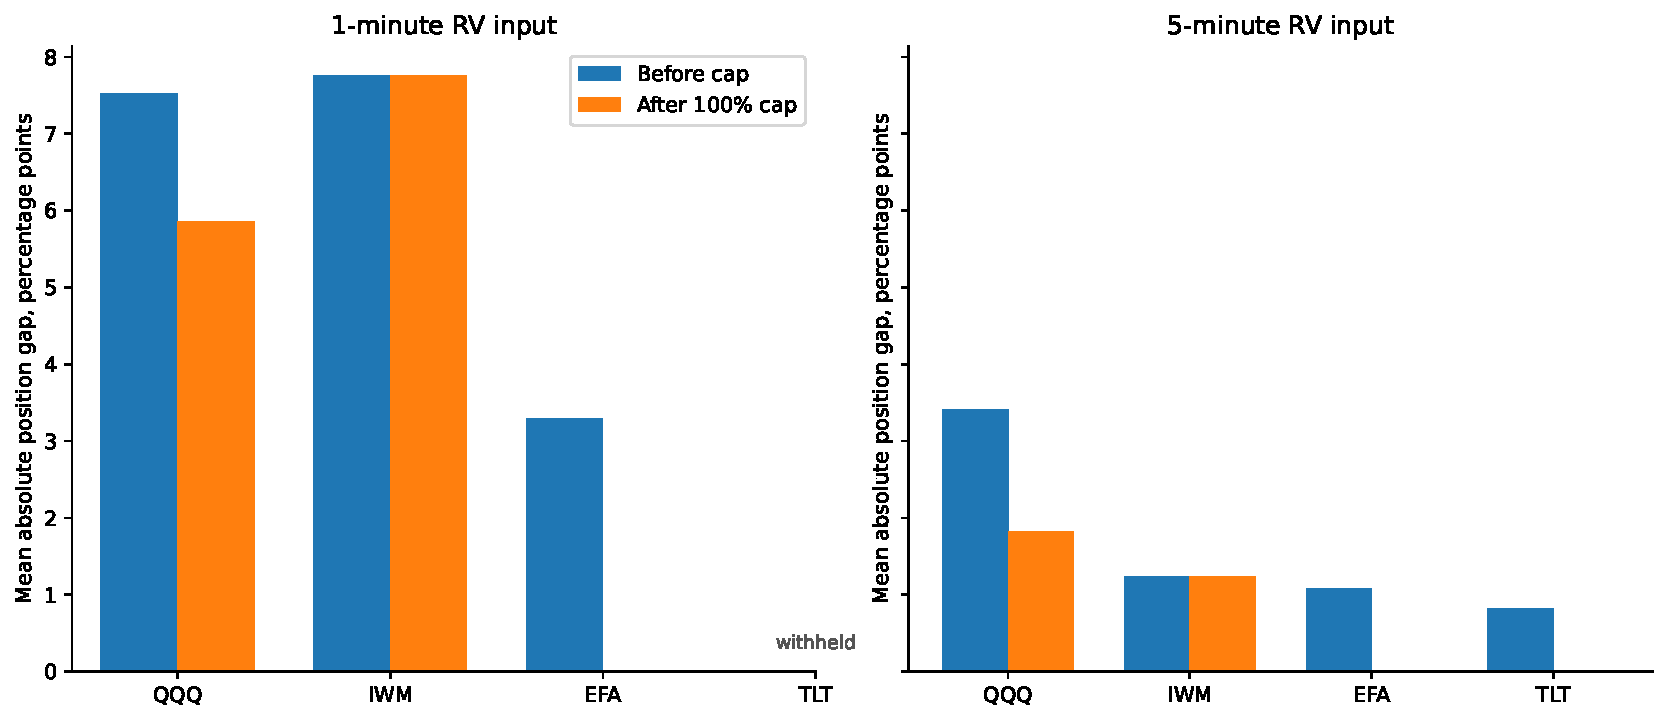
\includegraphics[width=\linewidth]{figures/breadth_cap_comparison.pdf}
\caption{Mean position gaps before and after the common cap. Both panels use the same vertical scale, measured in percentage points. The cap can hide most of the proposal gap for some funds, while leaving much more of it for others. TLT's incomplete one-minute comparison is explicitly withheld. A large percentage of masking must be read together with the actual uncapped gap. These are differences between rule inputs, not trading returns.}\label{fig:breadth-cap}
\end{figure}

\textbf{The category-B explanation is also fund-specific.} For QQQ at one minute, restoring B information leaves \BF{QQQ60BRVN} material RV dates. Using all modern condition information with legacy time leaves \BF{QQQ60CRVN}. Restoring B therefore does not explain QQQ in the same way as SPY.

This supports checking the full set of source fields and how they interact with the pipeline. It does not establish one economic cause for every fund or one universal category-based repair. The exact meanings of every field in the mounted sources remain a separate documentation question.

\textbf{Checks and complete reporting.} The export passed \BF{members} file-member hash checks, calendar and coverage checks, and daily correspondence and measurement checks. A separate result implementation recalculated \BF{checks} numerical values. It checked the smoothed rule through explicit weighted sums, separately implemented the block resampling and rejected a deliberately changed affected-date count.

Appendix~\ref{app:breadth} retains all fixed fund/grid/construction counts and their valid denominators. The supplied summary files also retain all three slope bands, all risk summaries and all specified block-length intervals. The follow-up shares the same historical source regime as SPY; these checks do not turn it into a test of a new regime or make either source verified economic truth.



\section{What the study tells us, and where it stops}\label{sec:limits}
The useful distinction is between agreement in the recorded information, agreement in the resulting volatility estimates, and agreement in the final proposed positions. Each needs its own check. A common cap can make the last quantities agree while concealing differences in the estimates that produced them.

The fixed practical warning criterion is met in this historical example. That makes the pipeline sensitive enough to deserve attention under the stated rule. It does not prove a new estimator, academic priority, the best cleaning rule or better investment performance. Earlier research already establishes measurement-induced apparent roughness and historical TAQ compatibility problems.

The historical sample is an important limitation. All five funds share the same source-overlap period. More funds do not provide a new market regime or a test of today's data. Time precision, condition coverage and market structure can change. Block-resampling intervals also rely on assumptions about this historical period; they are not guarantees for a different source regime.

The strict trade filter and approximate opening rule matter too. The filter deliberately asks a narrow question and excludes conditions retained by broader cleaners. Restoring category B is informative for SPY but does not uniformly resolve the other funds. A comparison of alternative cleaning rules would need a separately fixed study.

The modern source is a reference, not verified true integrated variance. Matching recorded rows is not the same as identifying unique economic executions. A lower H-tilde value does not identify hidden roughness, and a smaller investment-weight gap does not prove a better risk estimate.

Finally, the positions are calculated inputs rather than an investment backtest. We do not calculate realized returns, costs, overnight risk or execution outcomes. The original registered 1,250-day forecast comparison remains deferred because the required compatible source history is unresolved. This case study does not replace it with a shorter contest. An option implied-volatility surface is unnecessary for the present question and is not part of the evidence.

\section{Checks, reproduction and authorship}\label{sec:reproduction}
\subsection{What was checked}
Different checks address different possible mistakes. File hashes check whether exported files changed. Coverage checks compare the requested funds and sessions with what was produced. Independent calendar checks detect mistakes such as using a full-session interval count on an early-close day.

The daily RV/RQ calculations are compared between SQL aggregation and a separate NumPy construction. Recorded-row correspondence is checked separately. Two programs agreeing on RV would not, on its own, prove that they used the intended trading session or matching source records.

At the result level, a separate implementation recalculates \Fact{checksA10} original A10 values. The A11 check recalculates \Fact{checksA11} values and \Fact{overlaps} values that overlap A10. It uses a direct weighted sum to check the EWMA update instead of repeating the analysis's recursive calculation. It also rejects a deliberately altered policy output. The A13 checks are described in Section~\ref{sec:breadth}.

The mathematical appendix has separate checks of selected formulas, including normal moments, variance scaling, memory initialization and cap boundaries. These checks establish agreement for the stated cases and assumptions. They do not prove that every possible error is absent or that the assumptions hold for market data. Appendix~\ref{app:audit} records the checks and their limits.

\subsection{How numbers in the paper are connected to outputs}
The displayed research numbers and table cells are generated from recorded analysis outputs. A separate checker follows each number back to its specified source field and checks its transformation and printed value. A \emph{run ID} is a unique label for a recorded execution; Appendix~\ref{app:audit} and the repository use these labels to identify the relevant outputs.

This makes the calculations auditable without asking the reader to trust a manually typed table. The source code, file hashes and recorded configurations support reproduction. The data-free synthetic examples can be run without a WRDS account. Recreating the historical empirical results still requires the separately licensed input observations.

\textbf{Data availability.} The repository supplies original code, synthetic examples, aggregate research summaries and the manuscript. Raw trade records, licensed daily observations and private working Git history are excluded. Closed validation and final-period observations have not been used.

\textbf{AI and authorship disclosure.} Martin Valachy set the research direction, scope and goals. Codex implemented the computational pipeline, numerical checks, figures and draft. Human comprehension and independent human peer review are not asserted complete. Agreement between separate programs is computational checking, not human peer review. The paper is a working draft for honest undergraduate research review; it does not imply journal acceptance or work performed without AI assistance.

\section{Conclusion}
In this historical comparison, the way trade information is stored changes some volatility estimates and the investment positions proposed from them. Applying the same filtering code does not ensure that different data sources preserve the same information.

An upper position limit adds a second issue: similar final positions can hide disagreement between the underlying estimates. The additional funds make this conclusion more specific. QQQ retains substantial five-minute position differences, while EFA shows strong one-minute cap masking. Incomplete TLT histories are left unavailable rather than turned into apparent agreement.

The practical lesson is to check source information, daily measurements, smoothed estimates and capped positions separately. The study supports that audit procedure in the stated historical setting. It does not identify true market roughness, select a universally best sampling interval or demonstrate a profitable strategy.

